%%%%%%%%%%%%%%%%%%%%%%%%%%%%%%%%%%%%%%%%%%%%%%%%%%%%%%%%%%%%%%%%%%%%%%%%
%                                                                      %
%     File: Thesis_Appendix_A.tex                                      %
%     Tex Master: Thesis.tex                                           %
%                                                                      %
%     Author: Andre C. Marta                                           %
%     Last modified :  2 Jul 2015                                      %
%                                                                      %
%%%%%%%%%%%%%%%%%%%%%%%%%%%%%%%%%%%%%%%%%%%%%%%%%%%%%%%%%%%%%%%%%%%%%%%%

\chapter{Jet radius discussion}
\label{chapter:jetrad}

It is important to discuss if the radius of the jet that is used to reconstruct the boosted Higgs boson candidates ($R=0.8$) is the appropriate one. The question arises because in ATLAS boosted objects with $p_T\sim 200$ GeV are reconstructed using $R=1.0$ jets. In this work, we work with a CM energy of $100$ TeV and require that the two leading jets have $p_T>200$ GeV and use jets with $R=0.8$. It is necessary to understand if these jets are large enough to fully reconstruct the Higgs candidates. 

As a first approximation we compute the angle between the b quarks produced by the decay of a Higgs boson. We assume that the b quarks are massless and that the Higgs moves only in the transverse plane (perpendicular to the beam pipe) such that it has no longitudinal momentum and the angle between the b quarks is given by $\Delta\phi$. For $p_T(\text{Higgs})=200$ GeV, we get $\Delta\phi(b,\overline{b})=1.1$ which is smaller than the jet's diameter ($1.6$) and therefore the two b quarks can both be contained inside the jet and the Higgs boson fully reconstructed.

%\begin{table}
%	\centering
%	\begin{tabular}{ll}
%		\toprule 
%		$p_T(\text{Higgs})$ [GeV] & $\Delta\phi (b,\overline{b})$\\
%		\midrule
%		$200$ & $1.1$\\
%		\rowcolor{black!7} $300$ & $0.8$\\
%		$400$  & $0.6$\\
%		\bottomrule
%	\end{tabular}
%	\caption{oi}
%	\label{table:jet_radius}
%\end{table}

\begin{wrapfigure}{R}{0.5\textwidth}
	\centering
	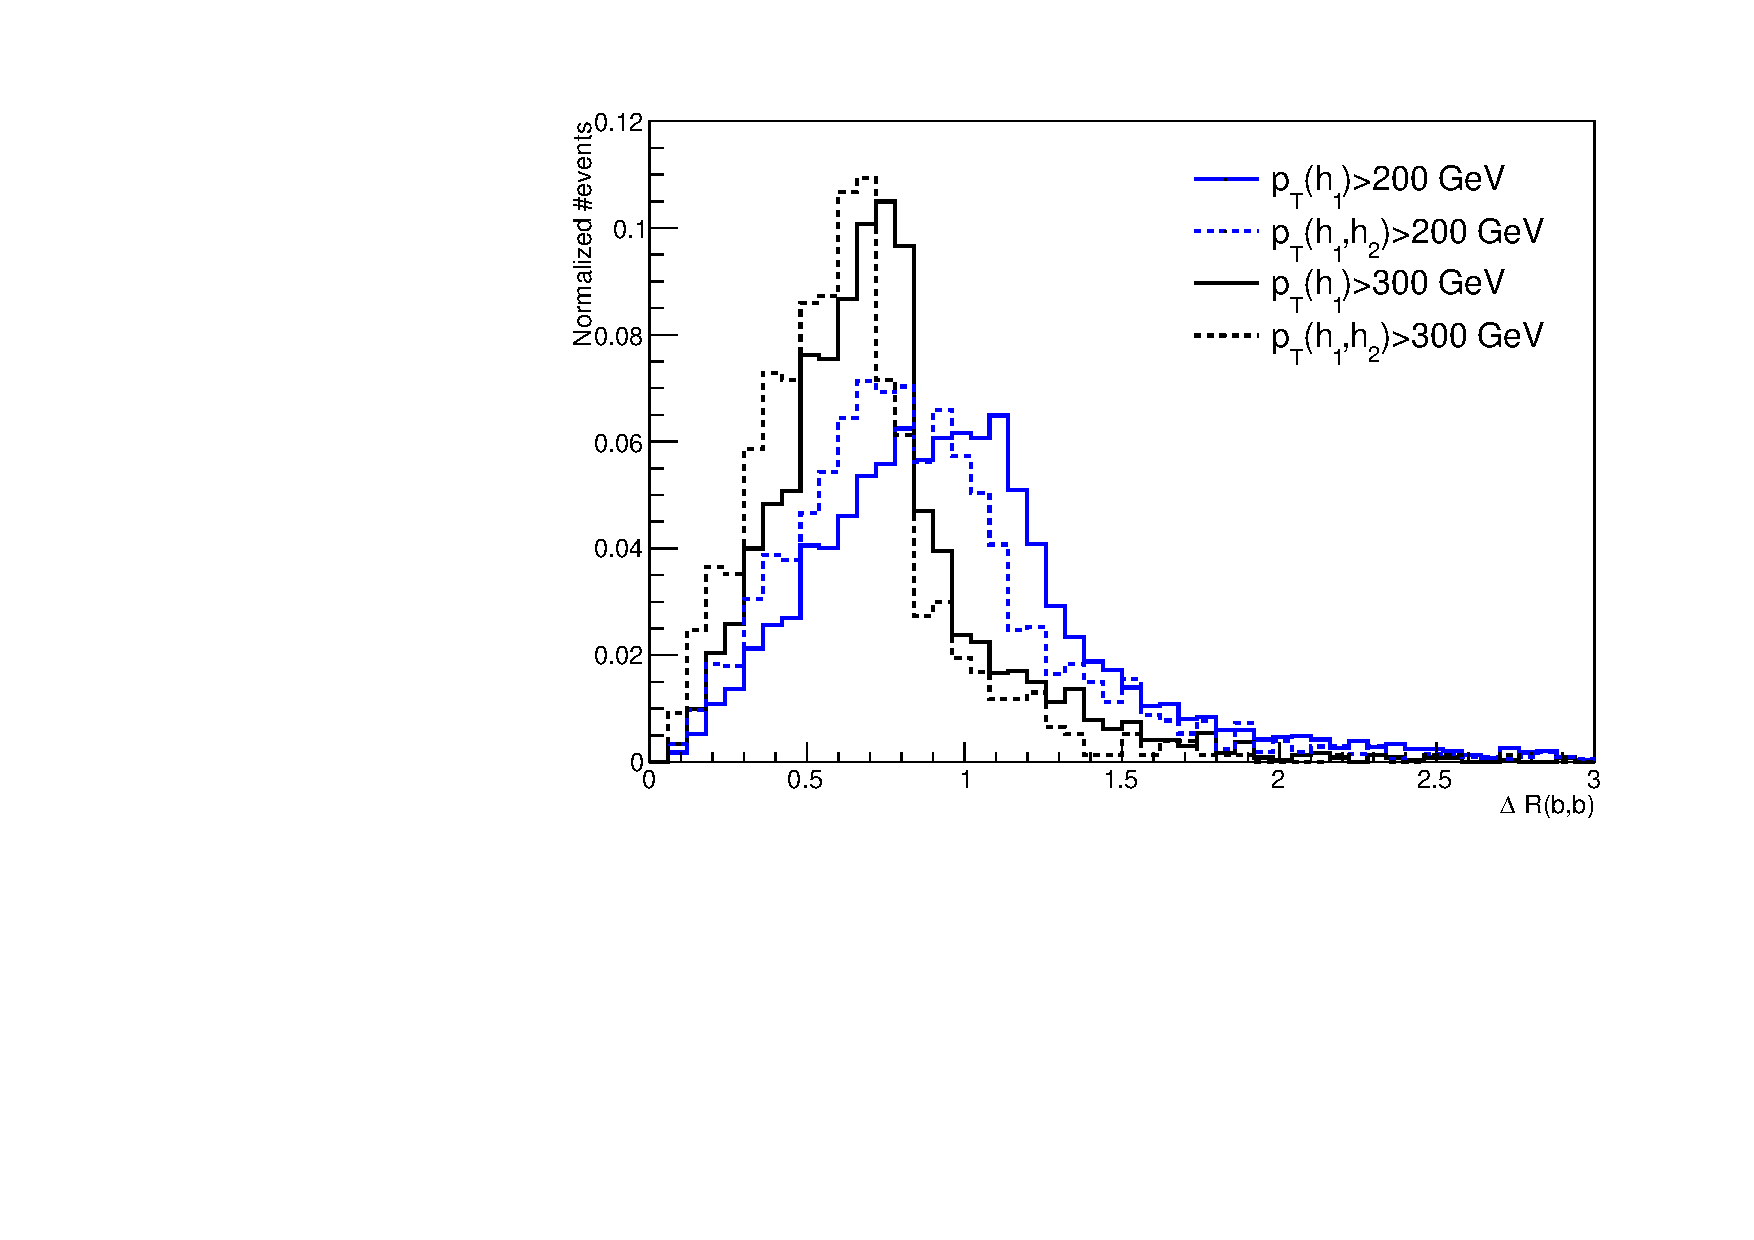
\includegraphics[width=0.5\textwidth]{./Figures/deltaR.pdf}
	\caption{\label{fig:deltaRbb} $\Delta R(b,\overline{b})$ distributions for $p_T(h_1)>200/300$ GeV (solid blue/black) and for $p_T(h_1,h_2)>200/300$ GeV (dashed blue/black).}
\end{wrapfigure}

Another test we can make is to compute the $\Delta R$ between the b quarks coming from the leading Higgs candidate with $p_T$ larger than a given value using truth level information. In figure \ref{fig:deltaRbb} we show the distribution of $\Delta R(b,\overline{b})$ for $p_T$ of the leading Higgs candidate larger than $200$ GeV (solid blue) and $300$ GeV (solid black). To obtain the dashed histograms we apply the $p_T$ to both Higgs candidates. The integral of the histograms between $0$ and $1.6$ gives an estimate of the fraction of signal we keep if we apply these $p_T$ cuts. For $p_T(h_1)>200(300)$ GeV we get that $93$($98$) \% of the signal has b quarks with $\Delta R <1.6$ and therefore can be fully reconstructed using a jet with $R=0.8$.



%\begin{figure}
%	\centering
%	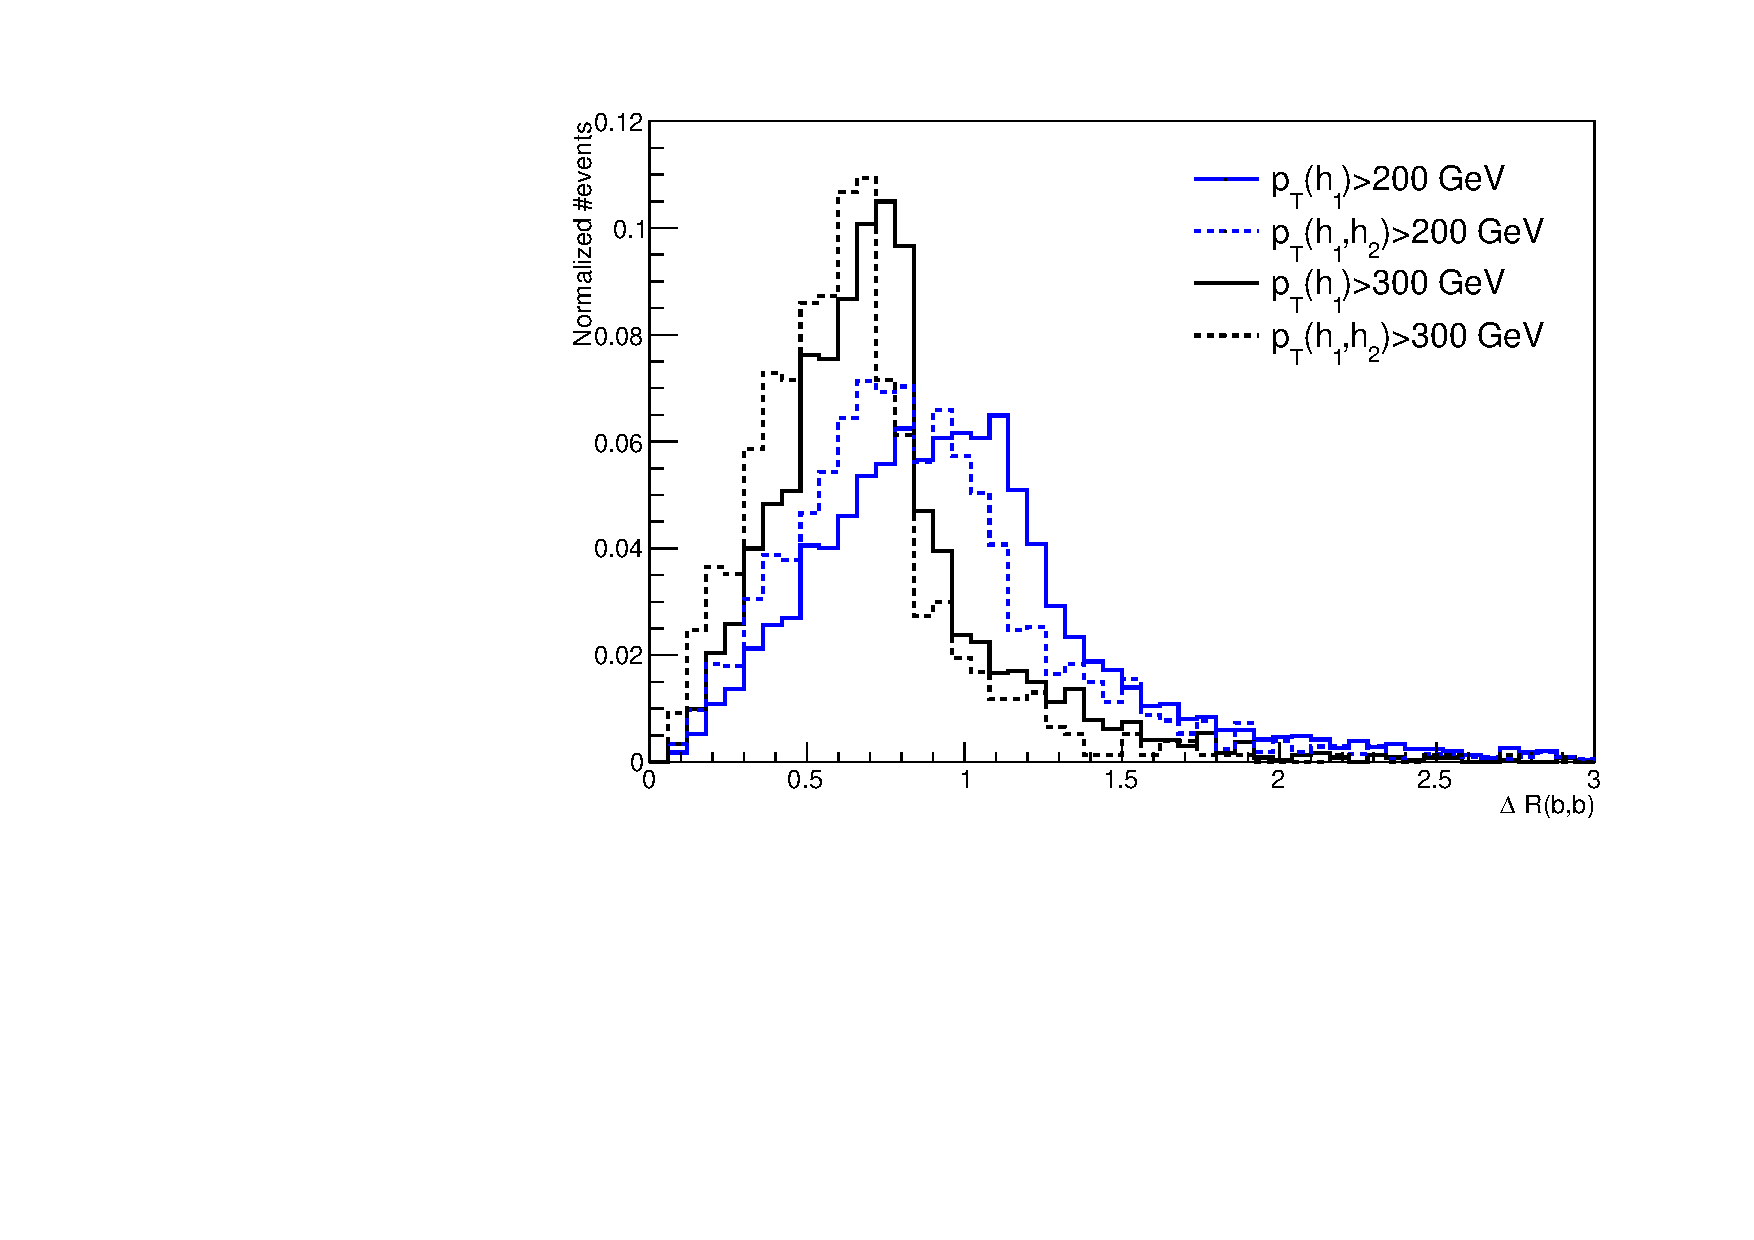
\includegraphics[width=.6\textwidth]{./Figures/deltaR.pdf}
%	\caption{oi}
%	\label{fig:deltaRbb}
%\end{figure}
